\section{Introduction}
\label{sec:intro}
Robotic technology is one of the pillars of modern society. Thanks to advances in information, electronic, and
mechanical fields, we can build and program machines to solve various tasks in different scenarios, e.g. industrial,
surgery, space missions etc. \newline In manufacturing, given their ability to reproduce the same movement over time
with an high level of accuracy and precision, robots are massively used to solve repetitive and dangerous activities
such as assembly, welding (Figure \ref{fig:welding}) and material handling    (Figure \ref{fig:material_handling}).
\begin{figure}[htb]
     \centering
     %\begin{subfigure}[b]{0.6\textwidth}
     %    \centering
     %    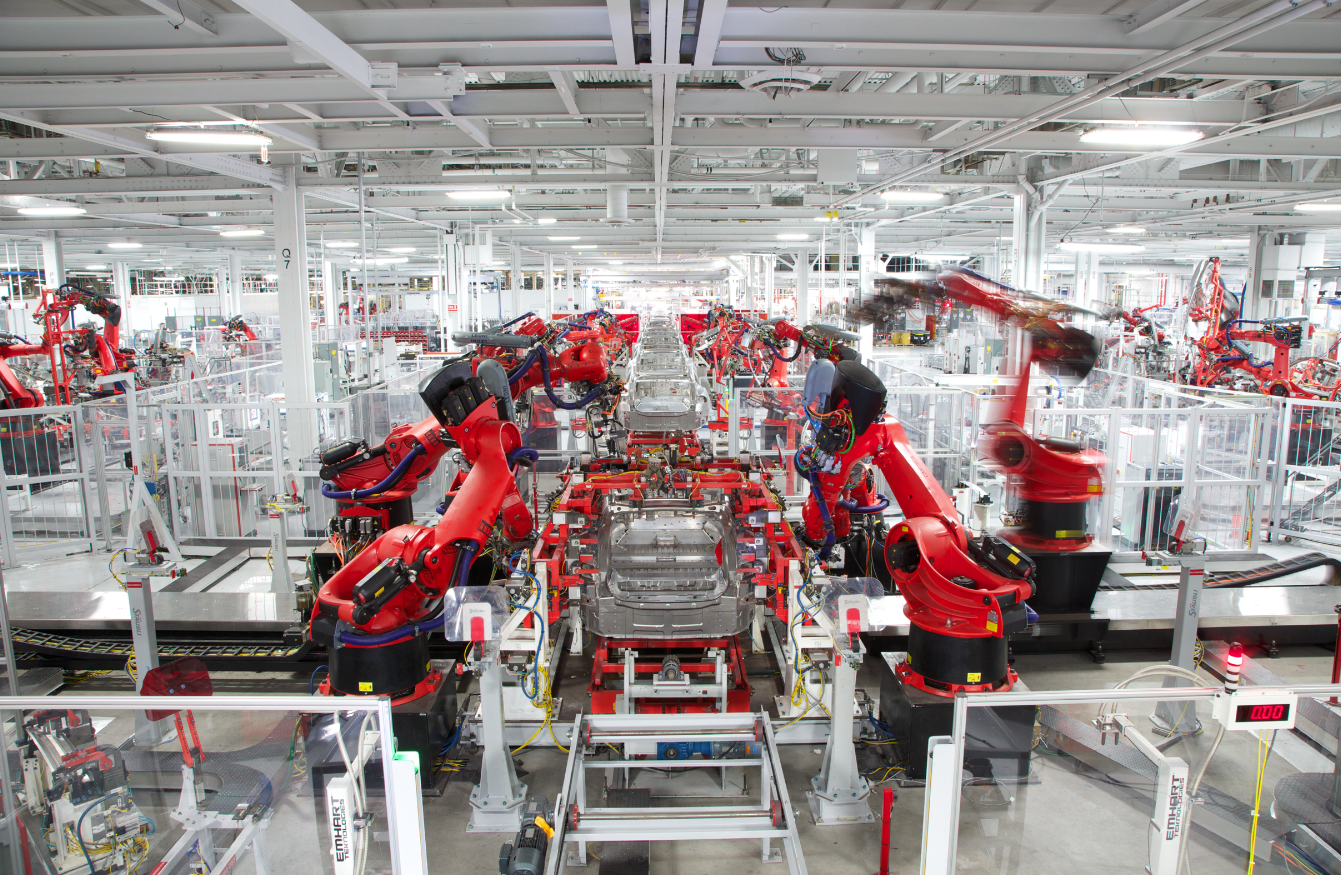
\includegraphics[width=\textwidth]{Figures/images/assembly.jpg}
     %    \caption{Robots involved in Tesla Assembly line}
     %    \label{fig:assembly}
     %\end{subfigure}
     %\hfill
     \begin{subfigure}[b]{0.45\textwidth}
         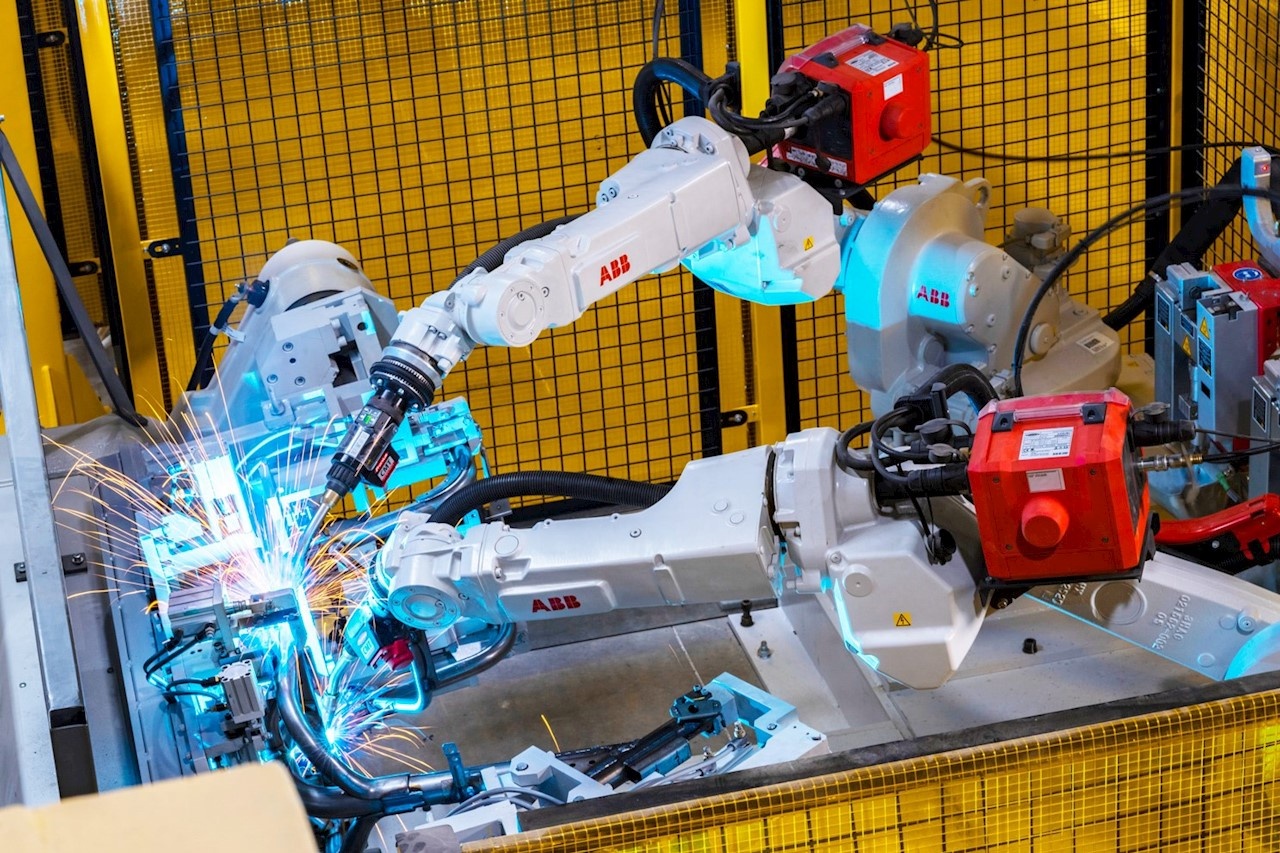
\includegraphics[width=\textwidth]{Figures/images/welding.jpg}
         \caption{Robots involved in arc welding operation}
         \label{fig:welding}
     \end{subfigure}
     \hfill
     \begin{subfigure}[b]{0.5\textwidth}
         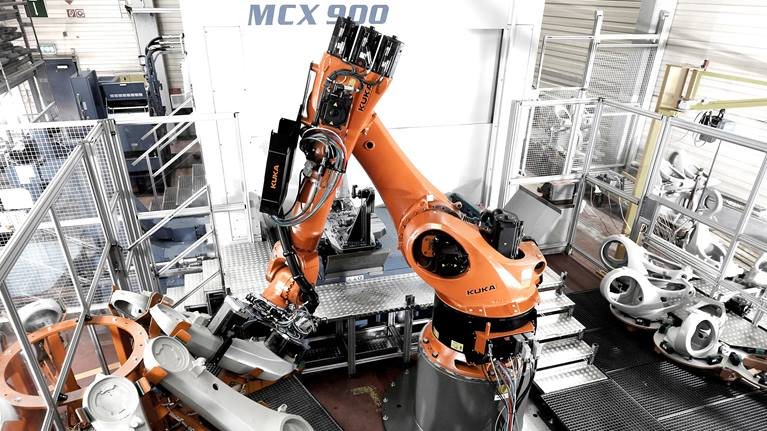
\includegraphics[width=\textwidth]{Figures/images/loading.jpg}
         \caption{Robot involved in loading operation}
         \vspace{0.5cm}
         \label{fig:material_handling}
     \end{subfigure}
    \hfill
    \caption{Industrial Robots: example of applications}
    \label{fig:industrial_robots_example}
\end{figure}


%Given improvements in control techniques and motion precision, robotic systems can reproduce very sensible movements
%needed, for example, in %surgery applications. \medskip \noindent \fcolorbox{red}{yellow}{%
%\minipage[t]{\dimexpr0.48\linewidth-2\fboxsep-2\fboxrule\relax} Inserire immagine Cooperation \endminipage} \medskip
\noindent While in the early day, robotic systems were constrained in isolated and known environments. Over the past few
decades, robots have been asked to solve tasks in dynamic and unknown/partially-known environments, where they must
\textbf{coexist} and \textbf{cooperate} with humans, while  solving different \textbf{dynamic} tasks (e.g. pick a
requested object, whose position is not known a priori). \newline The reason for the increasing demand for such
applications may be found in factors such as:
\begin{enumerate}[label=(\alph*)]
    \item The affirmation of the \textit{Industry 4.0} paradigm, in which the various phases of a factory are linked to
    each other and therefore the robots must be in communication with each other and be able to adapt to changes in the
    production phases.
    \item The spreading of \textit{social robots} (e.g. Pepper \cite{pepper}), that find their appeal in highly
    unstructured applications such as household or shop-recommendation systems.      
    \item The increasing availability of the so-called \textit{cobots} (e.g. Franka Emika Panda robot \cite{panda}),
    which are low-cost robots that allow the automation of light load processes (e.g. drilling, palletizing, polishing)
    while sharing the workspace with humans or other robots. Thanks to cobots, also small factories, that were left out
    from this automation process because of the high-cost of previous solutions, can now start to automate their
    production phases, contributing to increase the demand.
\end{enumerate}
In this scenario, the desired characteristics of such robotic systems are:\begin{enumerate*}[label=\textbf{(\alph*)}]
    \item The capability to exhibit \textit{``intelligent" behaviors} during the task execution in response to dynamic
    changes in the environmental condition (e.g. pre-grasping manipulation \cite{kalashnikov2018qt_opt}, motor failure
    and environmental uncertainties \cite{anne2021meta_learning_fast_adaptive}).
    \item The ability to easily \textit{adapt} to new tasks \cite{jang2022bc_z}. 
\end{enumerate*}
\newline These requirements can be difficult to obtain with typical robotic programming techniques based on hand-written
policy, and control techniques which require a careful analysis of the process dynamics, the building of an analytic
model, and finally, the derivation of a control law that meets certain design criteria
\cite{hafner2011reinforcement_in_feedback_controll}. This design process is tedious, and time consuming, especially when
\textbf{high-level perception systems} (e.g. camera, microphones, motion sensors etc.) are used to infer the state of
the environment (e.g. the unknown position of the desired object to pick with respect to the end-effector) and/or the
intention of the human operator. \newline In contrast, very relevant results have been obtained by leveraging
\textit{Learning Techniques}, which exploit \textbf{agent experience} or \textbf{expert demonstration}. Generally, the
former is referred as \textit{Reinforcement Learning} (RL) \cite{sutton2018reinforcement}, while the latter is referred
as \textit{Imitation Learning} (IL) or \textit{Learning from Demonstration} (LfD)
\cite{argall2009robot_learning_from_demonstration}. Both the approaches aim to obtain an artificial agent, that able to
perform correctly a task or a set of tasks by following a learned policy, however the way how this goal is achieved is
quite different. The main differences between RL and IL are related to presence/absence of a reward function, and the
presence/absence of expert demonstrations. \newline Indeed, in RL formalism \cite{kaelbling1996reinforcement_survey},
the learning procedure is based on a \textit{hand-designed reward function}, i.e. a measure of the quality of the
performed action with respect to the task to be executed (e.g. the distance between the current position and the target
one in a reaching task \cite{}), which drives the agent to produce a sequence of actions which maximize the reward.
While in IL formalism \cite{osa2018algorithmic}, the learning procedure is based on the minimization of a
\textit{loss-function} (e.g. Mean-Squared Error \cite{james2013introduction_to_sl}, Hinge-loss \cite{cortes1995support},
Kullback-Leibler divergence \cite{kullback1951information}), which guides the agent to reproduce/mimic the same actions
of the expert. \newline Regarding the possibility to exploit past experience, in RL literature, three approaches can be
found \cite{levine202rl_tutorial}:
\begin{itemize*}
    \item \textbf{\textit{On-policy}} Reinforcement Learning (Figure \ref{fig:onpolicy}), the trained policy is the same
    policy used to collect data, so, the only used past experience is related to the last policy rollout. These methods
    require a considerable amount of interactions to be trained \cite{}.
    \item \textbf{\textit{Off-policy}} Reinforcement Learning (Figure \ref{fig:offpolicy}), there are two policies, the
    behavior policy used to get experience, and the target policy, the policy to evaluate and improve. The target policy
    can exploit past experience during training. These methods are known to be more data-efficient \cite{}, although
    they still require interaction with the environment. 
    \item \textbf{\textit{Offline}} Reinforcement Learning (Figure \ref{fig:offline}), this setting is similar to the
    classic \textit{supervised learning approach}, where the target policy is trained via a \textit{static dataset} $D$,
    collected by an unknown policy $\pi_{\beta}$.  
\end{itemize*}
\begin{figure}[htbp]
     \centering
     \begin{subfigure}[b]{0.25\textwidth}
         \centering
         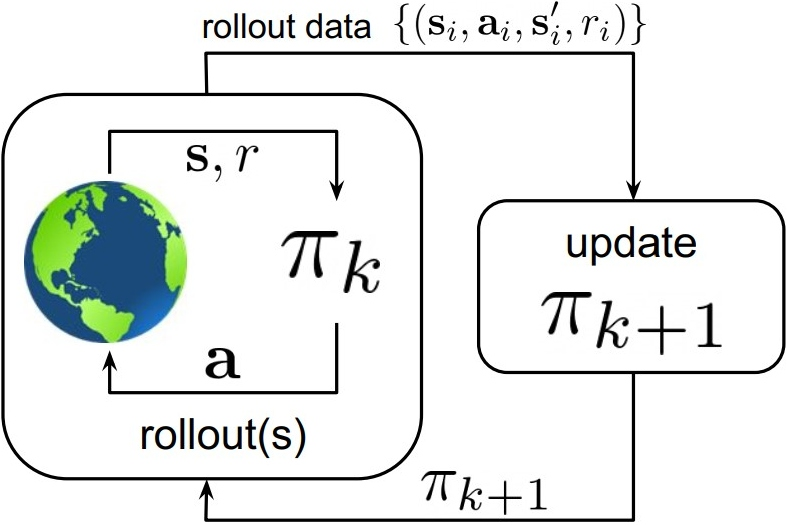
\includegraphics[width=\textwidth]{Figures/images/RL_methods/onpolicy.jpg}
         \caption{On-policy RL}
         \label{fig:onpolicy}
     \end{subfigure}
     \hfill
     \begin{subfigure}[b]{0.25\textwidth}
         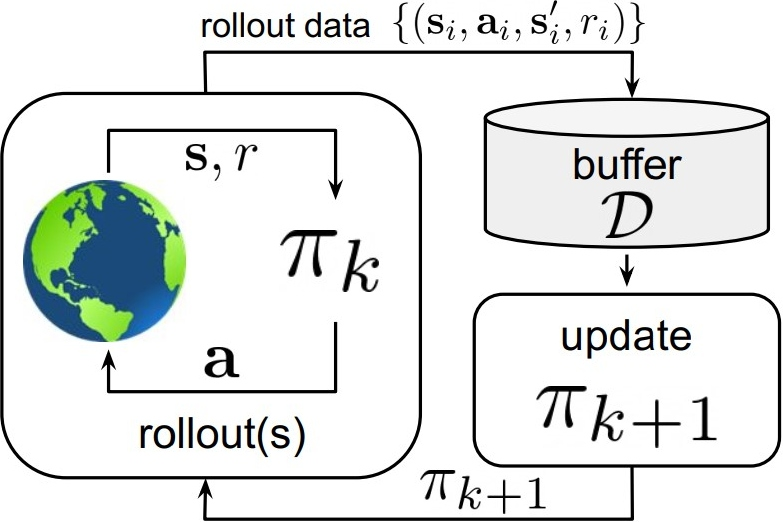
\includegraphics[width=\textwidth]{Figures/images/RL_methods/offpolicy.jpg}
         \caption{Off-policy RL}
         \label{fig:offpolicy}
     \end{subfigure}
     \hfill
     \begin{subfigure}[b]{0.35\textwidth}
         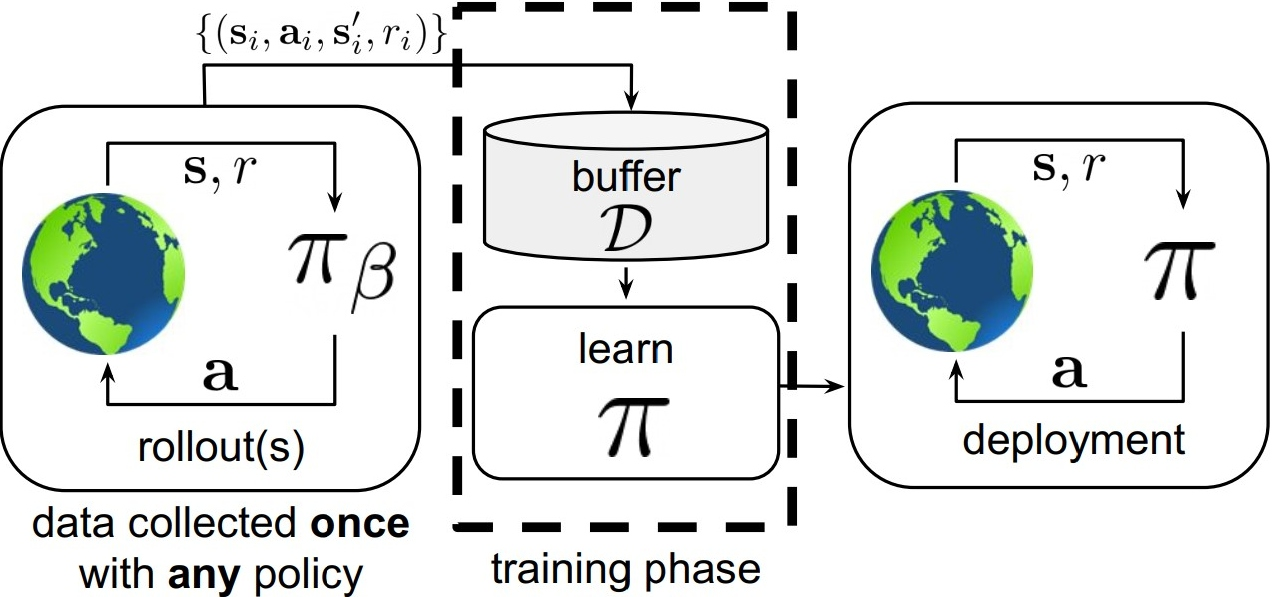
\includegraphics[width=\textwidth]{Figures/images/RL_methods/offline.jpg}
         \caption{Offline RL}
         \label{fig:offline}
     \end{subfigure}
    \hfill
    \caption{Graphical Representation of Reinforcement Learning Methods \cite{levine202rl_tutorial}}
    \label{fig:rl_methods}
\end{figure}


\noindent The need for a task-specific reward function, and the need for expensive and time-consuming training
procedures, are the main difficulties in applying such methods for real-world application
\cite{hussein2017imitation_learning_survey}. \newline As opposed to RL, in IL, the starting point for all the methods
(Figure \ref{fig:il_methods}), is a dataset $D$ containing expert demonstrations (e.g. trajectories of teleoperated
robot \cite{}, video of human pouring a liquid \cite{}). Based on the approach, the information contained in the dataset
is used in different way:
\begin{itemize*}
    \item \textbf{\textit{Behavioral Cloning}} (BC), the information contained in the dataset is used as \textit{ground
    truth}, i.e. the final learned policy mimics the same actions in the dataset \cite{}.
    \item \textbf{\textit{Inverse Reinforcement Learning}} (IRL), the demonstrations are used to learn a \textit{cost
    function}, that is subsequently used by an RL algorithm \cite{},
    \item \textbf{\textit{Generative Adversarial Imitation Learning}} (GAIL), combination of GAN \cite{} and IL, in this
    setting the agent, which acts as the Generator in GAIL, must produce a sequence of state transitions, such that
    Discriminator is not able to distinguish between generated transitions and demonstrated ones \cite{},
    \item \textbf{\textit{Learning from Observation}} (LfO), inspired by the fact that humans and animals are able to
    learn by just watching a demonstration, without knowing the underlaying performed actions (e.g. the joint position),
    then the aim of the artificial agent is to reproduce the observed behavior, starting from state-only demonstrations
    \cite{torabi2019recent_advances_lfo}.   
\end{itemize*}
\begin{figure}[htb]
    \centering
    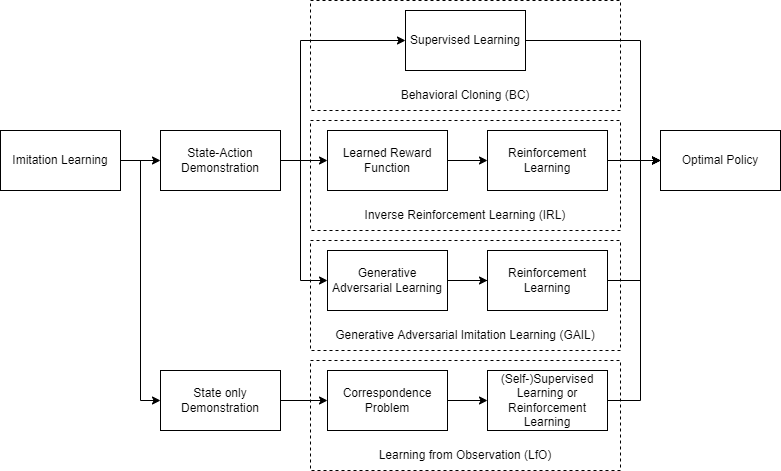
\includegraphics[width=0.9\textwidth]{Figures/images/il_taxonomy.png}
    \caption{Imitation Learning: Taxonomy and main components}
    \label{fig:il_methods}
\end{figure}


From Figure \ref{fig:il_methods}, it can be noted as IL and RL are strictly related, indeed, RL algorithms are used in
the training procedure of some methods, such as IRL, GAIL, and LfO. However, with respect to classic RL, IL allows to:
\begin{enumerate*}[label=\textbf{(\arabic*)}]
    \item bypass, or at least attenuate, the time-consuming exploration that would be required in a RL setting, 
    \item communicate, through demonstrations, a ``preference" for how a task should be performed.
    \item describe concepts that may be difficult to define formally or programmatically. \end{enumerate*}. As will be
explained in detail in Section \ref{sec:sota}, BC methods suffers of the \textit{compounding error} problem, since the
i.i.d. assumption that lays behind Supervised Learning is violated \cite{}. IRL was proposed to combine both the
data-efficiency of IL, to learn a reward function given the samples, and the exploration capability of RL, to attenuate
the \textit{compounding error} problem. However such methods have proved difficult to train. GAIL was proposed to reduce
the training complexity related to IRL, by framing the IRL problem as an Adversarial Learning problem, while the methods
improved both the performance and the efficiency of w.r.t. IRL methods, they showed poor performance when applied in
high-dimensional data, mainly due to the \textit{casual-confusion} problem \cite{}. LfO \cite{} was mainly proposed with
the aim to find a way to exploit state-only demonstrations, that are easy to obtain, and to collect. However, since
there is not any information about the true action,a way to measure the quality of prediction is needed. Moreover, the
\textit{correspondence problem}, i.e. how to map demonstration in human-space into the corresponding action in the robot
space, must be solved.     
\newline Despite all the open-challenges presented, IL was successfully applied for solving complex tasks, such as
driving a toy car \cite{codevilla2018end_to_end}, pick-and-place \cite{zhang2018deep}, and collaborative toolbox
assembly \cite{maeda2017probabilistic}, highlighting the high potential of such methods, which may justify an effort in
an attempt to resolve the gaps presented. A detailed description of the mentioned approaches will be given in
\textit{Section} \ref{sec:sota}, with an exhaustive comparison and description of the most recent and relevant methods.
%\noindent The need for a well-designed reward function, and the need for the system to interact with the environment
%during %the learning procedure, which is both time-consuming (e.g. in real-world experiments, at the end of each
%episode, the system %and the environment have to be put in the an initial state) and dangerous, are the main
%difficulties in using such approaches %in real-world application \cite{}. While the second drawback can be solved with
%the \textit{Offline RL}, 


